\documentclass{article}
\usepackage{graphicx} % Required for inserting images
\usepackage{amsmath}
\usepackage{amsfonts}
\usepackage{amssymb}
\usepackage{bm}
\usepackage{physics}
\usepackage{fancyhdr}
\usepackage{pgfplots}
\usepackage{siunitx}
\usepackage{braket}
\usepackage{mhchem}
\usepackage{chemfig}
\usepackage{gensymb}
\newcommand{\ve}{\mathbf}
\newcommand{\pa}{\partial}
\newcommand{\la}{\langle}
\newcommand{\ra}{\rangle}

\title{Fermi-Pasta-Ulam Problem}
\author{Lachlan Kan}
\date{March 2025}

\begin{document}
\maketitle
\section{Introduction}
Consider $N+1$ unit masses connected by springs of unit strength. We can write down the following 
Hamiltonian.
\begin{align}
    H=\frac{1}{2}\sum_{i=0}^Np_i^2+\frac{1}{2}\sum_{i=0}^N(x_{i+1}-x_i)^2
\end{align}
The boundary conditions are such that the "virtual points" $x_{N+1}=x_{-1}=0$. We will use this boundary condition for the remainder of this project. Notice that since we 
start counting from 0, our index goes up until $N$ and thus we end up with $N+1$
masses. Notice that for any $i$, there are two terms in the potential that concerns 
it. They are as follows 
\begin{align}
    (x_{i+1}-x_i)^2+(x_i-x_{i-1})^2
\end{align}
With this information,
 the equations of motion can be easily found via Hamilton's equations, where taking the 
 derivative with respect to $x_i$ amounts to focusing only on the segment from (2) that concerns the mass.  
\begin{align}
    \pdv{p_i}{t}&=-\pdv{H}{x_i}=x_{i+1}+x_{i-1}-2x_i\\ 
    \pdv{x_i}{t}&=\pdv{H}{p_i}=
    p_i 
\end{align}
Which leads to the following second order differential equation. 
\begin{align}
    \ddot{x}_i=x_{i+1}+x_{i-1}-2x_i
\end{align}
For each mass, we can ansatz a solution $x_i=A_ie^{j\omega t}$, where $j\equiv\sqrt{-1}$ and we
assume that they all share the same angular frequency $\omega$. Clearly this will only be the case when the system 
is oscillating in a normal mode. Hence we are solving for the normal modes. Using this ansatz, (5) becomes 
\begin{align}
    -\omega^2 A_i= A_{i+1}+A_{i-1}-2A_i
\end{align}
Writing out all the differential equations for $i=\{0,1,2,...,N\}$ and 
getting all the terms to one side, we obtain the following 
\begin{align}
    \begin{cases}
    0&=(\omega^2-2)A_0+A_{1}\\ 
    0&=A_0+(\omega^2-2)A_1+A_2\\   
    0&=A_1+(\omega^2-2)A_2+A_3\\ 
    \vdots \\
    0&= A_{N-1} +(\omega^2-2)A_N
    \end{cases}
\end{align}
This is now a linear system of equations with $N+1$ equations. 
To solve this, system, we must call upon linear algebra. Consider a vector with its component 
being that of the amplitudes. 
\begin{align}
    \ve{a}=
    \begin{bmatrix}
        A_0\\ 
        A_1\\ 
        \vdots\\ 
        A_{N-1}\\
        A_N
    \end{bmatrix}
\end{align}
Now we must construct the matrix. Notice that all the entries on the diagonal are 
$\omega^2-2$, since the coefficients on $A_i$ is $\omega^2-2$. On their neighbours $A_{i-1}$ and $A_{i+1}$, 
the entries are all $1$. Hence, the matrix is 
\begin{align}
    \ve{M}=\begin{bmatrix}
        \omega^2-2\ \ \ \ \ \ \  1\ \ \ \ \ \ \ 0\ \ \ \ \ \ \ 0\ \dots\ 0\ \ \ \ \ \ \ 0\ \ \ \ \ \ \ 0\\ 
        1\ \ \ \ \ \ \ \omega^2-2\ \ \ \ \ \ \ 1 \ \ \ \ \ \ \ 0\ \dots\ 0\ \ \ \ \ \ \ 0\ \ \ \ \ \ \ 0\\
        0\ \ \ \ \ \ \ 1\ \ \ \ \ \ \ \omega^2-2 \ \ \ \ \ \ \ 1\ \dots\ 0\ \ \ \ \ \ \ 0\ \ \ \ \ \ \ 0\\
        \vdots\ \ \ \ \  \ \ \ \ \ \ \vdots \ \ \  \ \ \ \ \ \vdots \\ 
        0\ \ \ \ \ \ \ 0\ \ \ \ \ \ \ 0 \ \ \ \ \ \ \ 0 \ \ \ \ \dots\ 1\ \ \ \ \ \ \ \omega^2-2\ \ \ \ \ \ \ 1\\
        0\ \ \ \ \ \ \ 0\ \ \ \ \ \ \ 0 \ \ \ \ \ \ \ 0\ \ \ \ \dots\ 0\ \ \ \ \ \ \ 1\ \ \ \ \ \ \ \omega^2-2\\
    \end{bmatrix}
\end{align}
This is a discrete Laplacian matrix of the tridiagonal form. Now, the system of (7) reduces to the following vector equation 
\begin{align}
    \ve{M}\ve{a}=\ve{0}
\end{align}
Or, equivalently expanded, we have the following 
\begin{align}
    \begin{bmatrix}
        \omega^2-2\ \ \ \ \ \ \  1\ \ \ \ \ \ \ 0\ \ \ \ \ \ \ 0\ \dots\ 0\ \ \ \ \ \ \ 0\ \ \ \ \ \ \ 0\\ 
        1\ \ \ \ \ \ \ \omega^2-2\ \ \ \ \ \ \ 1 \ \ \ \ \ \ \ 0\ \dots\ 0\ \ \ \ \ \ \ 0\ \ \ \ \ \ \ 0\\
        0\ \ \ \ \ \ \ 1\ \ \ \ \ \ \ \omega^2-2 \ \ \ \ \ \ \ 1\ \dots\ 0\ \ \ \ \ \ \ 0\ \ \ \ \ \ \ 0\\
        \vdots\ \ \ \ \  \ \ \ \ \ \ \vdots \ \ \  \ \ \ \ \ \vdots \\ 
        0\ \ \ \ \ \ \ 0\ \ \ \ \ \ \ 0 \ \ \ \ \ \ \ 0 \ \ \ \ \dots\ 1\ \ \ \ \ \ \ \omega^2-2\ \ \ \ \ \ \ 1\\
        0\ \ \ \ \ \ \ 0\ \ \ \ \ \ \ 0 \ \ \ \ \ \ \ 0\ \ \ \ \dots\ 0\ \ \ \ \ \ \ 1\ \ \ \ \ \ \ \omega^2-2\\
    \end{bmatrix}\begin{bmatrix}
        A_0\\ 
        A_1\\ 
        A_2\\
        \vdots\\ 
        A_{N-1}\\
        A_N
    \end{bmatrix}
    =
    \begin{bmatrix}
        0\\ 
        0\\ 
        0\\
        \vdots\\ 
        0\\
        0
    \end{bmatrix}
\end{align}
To solve this, we take the determinant of $\ve{M}$ and set it to 0. Then we can solve 
for $\omega$ directly. This method is easily implementable on python. However, it 
is computationally expensive and the computation time 
gets much longer with every mass added to the chain. 

\section{Nonlinear Perturbation}
We now perturb the spring potential by a nonlinear term. Let $\alpha$ be a small 
positive number. Applying the perturbation, the Hamiltonian is thus given by 
\begin{align}
    H=\frac{1}{2}\sum_{i=0}^Np_i^2+\frac{1}{2}\sum_{i=0}^N[  (x_{i+1}-x_i)^2 + \kappa (x_{i+1}-x_i)^{\gamma+1} ]
\end{align}
Where $\gamma=2$ or 3, depending on whether the perturbation is quadratic or cubic. 
Applying the same Hamilton equations and defining $\alpha\equiv\kappa(\gamma+1)/2$, we arrive at the following equations of motion 
\begin{align}
    \dot{p_i}&=(x_{i+1}+x_{i-1}-2x_i)+\alpha [(x_{i+1}-x_i)^\gamma-(x_i-x_{i-1})^\gamma]\\
    \dot{x_i}&=p_i
\end{align}
Here, we are interested in solving directly for the equations of motion. For computational purposes, 
it is best to condense all the momenta and position equations of the particles
into one state vector
\begin{align}
    \ve{v}=\begin{bmatrix}
        p_0\\ 
    x_0\\ 
    p_1\\ 
    x_1\\ 
    \vdots\\ 
    p_N\\ 
    x_N
    \end{bmatrix}
\end{align}
If we denote $\ve{v}=v^\mu$ where $\mu=\{ 0, 1, 2, ..., 2N+1\}$, 
then an even $\mu$ denotes momenta  and an odd $\mu$ denotes position.
From (15), we can specify the initial conditions by specifying $\ve{v}(0)$.
Similarly, we can construct a vector 
that encodes the time evolution of the state vector 
\begin{align}
    \dot{\ve{v}}=\begin{bmatrix}
    \dot{p}_0\\ 
    \dot{x}_0\\ 
    \dot{p}_1\\ 
    \dot{x}_1\\ 
    \vdots\\ 
    \dot{p}_N\\ 
    \dot{x}_N\\ 
    \end{bmatrix}
\end{align}
Where the time derivatives $\dot{p}_i$ and $\dot{x}_i$ can be found in (13) and (14) respectively. In Python, 
we can solve the system by creating a function that generates the evolution vector, 
and then passing the function (not the evolution vector itself, but the function that generates it), as well as the initial conditions 
$\ve{v}(0)$ on to 
scipy for solving. Since there is a nonlinear term to the differential equations, 
it is best to choose the Backwards Differentiation Formula (BDF) method to solve the system. 
A way to check for correctness of the code is to use only two masses and set 
$\alpha=0$. We can then 
displace the masses identically and release from rest. If this results in a normal mode, then the code is likely to be correct.

\section{Modal Spectra}
For any given system, it should be well known that there exists the same number of normal modes 
as its degrees of freedom. The mode spectra of the FPU oscillator can be found as the spatial Fourier sine 
transform of the displacement. The discrete Fourier coefficient $\phi_{ik}$ for the 
$i-$th particle in the $k$-th mode is as follows
\begin{align}
    \phi_{ki}=\sqrt{\frac{2}{N+1}}\sin\frac{ik\pi}{N+1}
\end{align}
We can thus construct the matrix $\phi_{ki}$ where the rows represent modes and 
columns represent particles. If we extract only the displacement from the state vector
and write out all its time evolution on the rows, then we obtain 
\begin{align}
    d_{it}=\begin{bmatrix}
        x_0(0)& x_0(t_1) & x_0(t_2) &\cdots \ \  x_0(t_f)\\ 
        x_1(0)& x_1(t_1) & x_1(t_2) &\cdots \ \  x_1(t_f)\\ 
       \vdots& \vdots & \vdots & \vdots\\ 
        x_N(0)& x_N(t_1) & x_N(t_2) &\cdots \ \ x_N(t_f)\\ 
    \end{bmatrix}
\end{align} 
We can thus find the discrete sine transform via the following well known formula 
\begin{align}
    a_{kt}=\sqrt{\frac{2}{N+1}}\sum_ix_i(t)\sin{\frac{ik\pi}{N+1}}=\sum_ix_{i}(t)\phi_{ki}
\end{align}
Notice the $t$ in the subscript means that we must apply the transformation across 
all time. Notice that we sum across all $i$, the index that the two matrices share. 
This "summing over repeated index"
is equivalent to the matrix product. Since $x_{i}(t)$ is discretised by $d_{it}$,
 the discrete Fourier coefficients for every point in time $t$ can be found by 
the following product 
\begin{align}
    a_{kt}=\phi_{ki}d_{it}
\end{align}
This can be easily calculated in Python by the $@$ operator, and has components of the time 
evolution of each mode. We can easily find the momenta modes by constructing the same matrix 
in (18) but with momenta, and projecting that onto the basis matrix $\phi_{ki}$, which yields 
the Fourier sine transform of momenta.

\subsection{Excitation of Modes}
To excite a certain mode, say the $k$-th mode, 
all we have to do is initialise the state vector 
in a way such that all the masses'
the initial displacements matches up
 exactly with the Fourier coefficient $\phi_{ki}$ in that $k$-th mode (Each mass
 will have a different initial displacement that corresponds to the mode). When the initial conditions are set up this way, the mode spectra 
will show a large amplitude for the desired mode $k$ and zero amplitude
 for the other modes.
Under nonlinear perturbation, 
the amplitude will "spread" from 
the $k$-th mode to the other modes, 
resulting in high amplitudes in the other modes over time. This contrasts with the linear case, 
whereby if the initial conditions are set up perfectly, 
only one mass will be excited for all time.
\section{Elementary Results}
Here are some elementary results and examples from the Python code, implementing the methods outlined in the previous sections.
\subsection{Quadratic Perturbation}
Here we will demonstrate the results when $\gamma=2$, which corresponds to the FPU-$\alpha$ problem.
\subsubsection{Testing with a Known Case}
To test the code, we first run it with $\alpha=0$ (no nonlinearity - a known case) with two masses 
starting with equal displacement. We obtain figure 1.
Notice that their displacements are identical. We have reached a normal mode. This is 
a known case, and we can be more confident that our solver is correct.
\subsubsection{Four Masses}
We can now examine more interesting cases. Consider 4 masses under quadratic perturbation. 
Here we have set $\alpha=1/6$ and displaced them initially with slightly different displacements, as shown in figure 2.
\subsection{Fifty Masses}
We will test 50 masses displaced identically at the start, released from rest. The plot, 
shown in figure 3 is beginning to look 
like that of a continuum. The small plot however, does not do the system justice since 
its amplitudes of oscillation are somewhat muted due to the sheer volume of masses needed 
to be fit into the small plot.
\subsection{Mode Spectra}
Here we will deal with the mode spectra part of the simulation.
\subsubsection{Exciting the First Mode}
Here, we will initialise the initial 
conditions such that they match up with the $k=1$ mode. 
Again, we will be dealing with 4 masses and testing with no nonlinearity. This results in 
figure 4. Notice that all other modes are 0 except for the $k=1$ mode. This is what we expect. 
We can now see what happens when there exists some nonlineariy, say $\alpha=1/4$. This results in 
figure 5. Notice that immediately, some Fourier amplitude gets 
"transferred" into the second mode. The $k=1$ mode is gradually decreasing in Fourier amplitude 
and the $k=2$ mode is gradually increasing. It may be interesting to run the simulation for a longer 
period of time to see what this leads to. Perhaps there exists a state where the decrease and 
increase stops and the system reaches equilibrium.
\subsubsection{Arbitrary Initial Conditions}
Here we will impose upon the system of 4 masses an arbitrary set of initial conditions, with $\alpha=1/4$ and 
observe the behaviour. This results in figure 6. Notice that one mode still dominates over the other, however 
the oscillations are now a combination of the modes.
\subsection{The Paradox}
In the modal spectra plots, we see that the first (excited) mode gradually decreases
in Fourier amplitude and the rest has its Fourier amplitudes gradually increase.
It may be tempting the think that if we let the simulation run long enough,
 that there will 
be a stable point where all the modes balance and the Fourier amplitudes do not change. In other words, 
the system will thermalise. However, our results shown in figure 7 tells a different story. Here, 
we run a much longer and large scale simulation, with $\alpha=0.6$ and 32 masses for a max time of 
36000 to observe the long term behaviour of the system. 
We also start the simulation by imposing initial conditions that excite mode $k=1$. 
 we observe the classic FPU paradox - 
instead of equipartitioning (same amplitude for all modes in equilibrium), 
the modes (major trends) oscillate. Mode 1 starts decreasing and 
mode 2 increases, but after sufficient time, mode 2 will star
 decreasing and mode 1 will increase again. 
This periodic behaviour was the original paradox, discovered by Fermi, Pasta and Ulam. 
In this simulation, the maximum Fourier amplitude for mode 1 decreases every major cycle.
We also compute the 
spectral energies for the system, shown in figure 8. Here we see the same phenomenon 
in terms of the energy - the energies gets 
periodically transferred from mode to mode. In the beginning,
 mode $k=1$ (the mode we excited initially) has the most energy. Later, 
other modes take over as having the highest energy. This "highest energy mode" is transferred 
between modes $k=2,3,4,...$ one by one until eventually, mode $k=1$ 
gains the most energy again, and the cycle continues. 
This raises the question of whether or not there is a bigger cycle, or does 
the system truly thermalise for large enough times. 
Unfortunately, this simulation was already heavy for the Macbook and the system is 
nowhere near thermalising. We can only conclude that even if the system thermalises,
the timescales required is too large to simulate on a typical computer. 

\subsection{Analogous Autoparametric Systems}
The traversal between modes is analogous to an autoparametric oscillator. 
Consider a mass attached to a spring, where the spring is hung from a ceiling and 
is free to swing in a plane, resulting in a mix between spring and pendulum motion. 
Such a system is "autoparametric", meaning that the mass will first trace out 
the spring motion, bobbing up and down, and then soon become pendulum-like,
 swinging side to side. Over time, the 
spring motion transforms into the pendulum motion and back, 
indefinitely.
The spring and pendulum motion can be 
thought as two different modes of which the system travels between.
\section{Comparing with the FPU Paper}
The orignal paper by FPU, published in 1955 computed the results for 
$N=32$ and $\alpha=1$. The recurrence time (time measured from the midpoint of 
the first "bump" to the midpoint of the second "bump") found was slightly over 
$14000$ (the exact value is not known since the results are presented
 on a hand drawn graph, and we need to infer roughly from that the recurrence time). When running the Python script 
under these conditions, we obtain a recurrence time of 13500. This gives an error of 
$~3.5\%$, 
which is not bad for our simulation. 
\section{Shannon Entropy}
Up until now, our metric of "thermalisation" and "equipartitioning" has been to just 
look at the energy plots and see if all the modes have equal amplitude. While this 
is a good way of gaining intuition, it is not the most rigorous way. To get a proper measure of how close the system is to thermalising, we need to introduce the notion 
of Shannon Entropy. Consider a series of events $X_i=\{X_0,X_1,X_2,...X_i\}$, and its associated set of 
probabilities $P(X_i)\equiv P_i$. A metric of "surprise" can then be constructed for these 
probabilities - a high probability means low surprise (it will probably behave as expected), 
while a low probability means high surprise. Moreover, a probability of 1 means no surprise whatsoever (it is guaranteed to behave as expected), 
while a probability of 0 is infinitely surprising in that there is no way to predict what happens next. One such function is the 
logarithm, $-\ln (P_i)$. This behaves as we expect, with $-\ln1=0$ and $-\ln0\to\infty$ from the right. The function 
is also decreasing, which fits our inverse proportional-esque expectations. Undoubtedly, 
the amount of information needed to specify a state $X_i$ is tied to this negative logarithm, since 
the more unexpected things are, the more information needed to specify the thing 
(ex. if your flight is on time as expected, 
then there isn't any new information I need to tell you. 
However, if your flight is unexpectedly delayed, 
then I will have to tell you some new information. Hence the
 "surprise event" itself carries 
new informaion that needs to be conveyed. 
In other words, the amount of information is tied to 
the surprising-ness of the event). To figure out the overall amount of information needed 
to convey an event, we simply weigh the surprising-ness by the overall probability. This is 
because if an event is more probable, then it will occur more times, and vice versa. If 
an event occurs more times, then more information will be needed to specify that event. Hence, 
the information needed $S_i$ is given by 
\begin{align}
    S_i=-P_i\ln(P_i)
\end{align}
For the overall amount of information needed to 
specify the whole set of events, we simply sum $S_i$ over all events $X_i$ to obtain $S$, 
the Shannon entropy 
\begin{align}
    S=-\sum_{i}P_i\ln(P_i)
\end{align}
Which represents the amount of information needed to specify the set of 
events $X_i$ by taking into account 
the rates of occurance and "surprising-ness". We can now apply this concept to the 
FPU problem. Here, the probability of observing each mode 
(think of seeing each mode as its own distict event) $k$ is given by $E_k/E$, where $E$ is the 
total energy. This is because the likelihood
of observing any given mode is directly linked to its energy. For example, 
if we excite the first mode, then it will have the most energy and dominate the system, 
hence it is very likely that we will observe the first mode when observing the system.
The Shannon entropy for any given mode 
is then 
\begin{align}
    S_k=-\frac{E_k}{E}\ln(\frac{E_k}{E})
\end{align}
And the total Shannon entropy at any given time can be obtained similarly by summing over all $k$
\begin{align}
    S=-\sum_k\frac{E_k}{E}\ln(\frac{E_k}{E})
\end{align}
Consider a system of $N+1$ masses (and thus $N+1$ modes). If the system has thermalised, 
then we'd expect $E_0=E_1=...=E_N$, and 
the only way for this to happen is such that 
\begin{align}
    E_k=\frac{E}{N+1}
\end{align}
Where the energy is evenly divided between the $N+1$ modes. Using (24), 
we can now find the total Shannon entropy $S_T$ of a thermalised system.
\begin{align}
    S_T&=-\sum_{k=0}^N\frac{E/(N+1)}{E}\ln(\frac{E/(N+1)}{E})\\ 
    &=\sum_{k=0}^N\frac{1}{N+1}\ln(N+1) = \frac{N+1}{N+1}\ln(N+1)\\ 
    &= \ln(N+1)
\end{align}
o measure how close a system is to thermalising, we can then compare the Shannon entropy of its incumbent state 
to the thermalised Shannon entropy. To show that this is the maximum Shannon entropy the system can attain, 
we consider the case $N=1$, with 2 masses. Suppose the energy is split unevenly, where 
\begin{align}
    E_0&=\frac{1}{2}(1+\xi)E\\ 
    E_1&=\frac{1}{2}(1-\xi)E
\end{align}
Where $-1\leq\xi\leq1$ and $\xi=0$ represents the thermalised, equipartitioned case where the energies are equal.
It can be shown that $E=E_0+E_1$, since adding together (29) and (30) naturally leads to the cancelling out 
of the $\xi$ terms. The Shannon entropy for the system is given by
\begin{align}
    S=-[\frac{E_0}{E}\ln(\frac{E_0}{E})+\frac{E_1}{E}\ln(\frac{E_1}{E})]
\end{align}
Rewriting it in terms of (29) and (30) gives us 
\begin{align}
    S&=-[\frac{(1+\xi)E/2}{E}\ln(\frac{(1+\xi)E/2}{E})+\frac{(1-\xi)E/2}{E}\ln(\frac{(1-\xi)E/2}{E})]\\ 
    &=-\frac{1}{2}[(1+\xi)\ln(\frac{1+\xi}{2})+(1-\xi)\ln(\frac{1-\xi}{2})]
\end{align}
Now we find the $\xi$ that leads to the maximum $S$. Notice that $\xi=\pm1$ (all energy in one mode, ie. one mode is excited) leads to $S=0$, and $S$ must be 
positive because $|\xi|<1$ makes the $1\pm\xi$ always positive, and the fact that $(1\pm\xi)/2<1$ means that 
the logarithms will always be negative. Thus, multiplying everything by $-1/2$ makes the whole expression positive.
To get between the zeroes at the endpoints,
 the function must have at least one critical value. Therefore, in 
the case that there only exists one critical value, it must result in a maximum. Let us now find the 
maximum    of (33). This can be easily done by differentiating and setting the result to zero. 
\begin{align}
    \dv{S}{\xi}&=-\frac{1}{2}\ln(\frac{1+\xi}{1-\xi})=0 \implies \boxed{\xi=0}
\end{align}
Which tells us indeed that the maximum Shannon entropy is achieved when $\xi=0$. 
We can expect that the excitation of any given
 mode will put the system at $S=0$.
With this intuition, we can now 
examine the general case of $N$ masses. We can think of this problem as "maximising the Shannon entropy 
under the constraint that all energies must add up to the total energy",
 and treat it with Lagrange multipliers. For this, we will make use of two functions - 
one for the Shannon entropy from (24), and one for the total energy constraint function. 
\begin{align}
    S&=-\sum_k\frac{E_k}{E}\ln(\frac{E_k}{E})\\ 
    C&=\sum_kE_k=E
\end{align}
Where $S$ can be thought of as an $N+1$ dimensional surface (1 dimension for every $k$). 
Similarly, the constraint $C$ will exist in the same space, imposing 
its restrictions upon the Shannon entropy. 
To make things easier, we will re-introduce our notation of 
$P_k\equiv E_k/E$ and make the change in variables. Our equations now read 
\begin{align}
    S&=-\sum_kP_k\ln{P_k}\\
    C&=\sum_kP_k=1
\end{align}
The last equation can be interpreted as the fact that
 adding together all of probability space must result in a total probability of 1. 
We can now implement the Lagrange multiplier method, which states that $\nabla S-\lambda\nabla C=0$, 
where $\lambda$ is the Lagrange multiplier. We now find the gradients. 
\begin{align}
    \nabla S&=-\sum_k\pdv{(P_k\ln P_k)}{P_k}\hat{P_k}=-\sum_k(\ln P_k+1)\hat{P_k}\\ 
    \nabla C& =\sum_k\pdv{P_k}{P_k}\hat{P_k}=\sum_k\hat{P_k}
\end{align}
Where $\hat{P_k}$ are the unit vectors associated with each degree of freedom $P_k$ that the surfaces resides in. 
Hence we obtain the following expression 
\begin{align}
    \sum_k[-(\ln P_k+1)-\lambda]\hat{P_k}=0
\end{align}
Notice that for the result of any general sum (nontrivial cases where the terms don't cancel out)
 to equal 0, the summand must all be 0. We can now say that for any $k$, 
\begin{align}
    -(\ln P_k+1)-\lambda=0\implies P_k=\frac{E_k}{E}=e^{-(\lambda+1)}
\end{align}
Notice how $P_k$ is independent of $k$. Since $P_k$ is just a scaled version of $E_k$, we can 
also say that $E_k$ is independent of $k$. This means that all the energies are the same, 
as there are no variation of energy between the mode number $k$. We can thus say that 
\begin{align}
    E_0=E_1=E_2=\dots=E_N=Ee^{-(\lambda+1)}
\end{align}
Which to be true, must satisfy the condition that the energy is distributed evenly, or mathematically 
\begin{align}
    E_k=\frac{E}{N+1}
\end{align}
Hence it can now be said that the maximum of the Shannon entropy must be a result of 
the equipartitioning of energy between modes. In other words, the Shannon entropy will always be less than $S_T$ where 
energy is not equally spread.  We can expect that the Shannon entropy will climb as the energy is distributed among the modes. 
We can plot $S/S_T$ as a function of time and observe its evolution. If the ratio climbs to and settles at 
1, then that means the system has thermalised (ie. ergodic). If $S/S_T<1\ \forall \ t$, then it confirms that the system never 
thermalises. However, this requires the computation power to simulate behaviours of the long term ($t\sim10^8$), 
which is not always realistic for regular computers.
\newpage 
\subsection{Results for Shannon Entropy}
We can now implement equation (24) into Python, and present some findings.
 The label on the $y$-axis is a misnomer. 
It should be $S/\ln(N+1)$ instead of $S/\ln N$. This is a relic
from a bug that set $E=\ln N$ that was fixed before. 
\subsubsection{Short Term}
We let the simulation run until $t=3\times10^3$ on a relatively small sample size ($N=20$) to obtain figure 9. Notice that $S/S_T$ indeed 
begins from 0 and slowly rises. However it never reaches 1 in the alotted time, 
meaning that in the time given, the system has not yet thermalised. It is interesting to note though, 
that the steady upwards trend is promising.
\subsubsection{Long Term}
We now let a simulation with the same number of masses run until $t=5\times10^6$ to observe the long term effects.
 We see that the upwards trend 
still exists very early on, but reaches a maximum of around 0.8 and stops increasing. After that, it shows a slow but clear decreasing trend, indicating that 
the energy is once again slowly being concentrated into one of the modes. 
\subsubsection{More Masses}
We are now interested in the case of many masses, say 100. The result is shown in figure 11.
We see that the Shannon entropy rises initially, as we expect. However, it soon stops and goes the other way. 
For longer times, it displays oscillatory behaviour about $S\approx0.4$ and never seems to settle into equipartitioning. 
\subsection{General Observations}
After running many more simulations for times $\sim10^3-10^6$ on varying numbers of masses,
we notice that the normalised Shannon entropy never reaches or shows any signs of 
steadily reaching 1 in the long run. All trials have resulted in behaviours of two kinds: 
the first is reaching a plateau somewhere below 1, and the second is oscillations around some point below 1. 
It certainly looks like, at least at these timescales, 
 that the system has a certain "stable state" which it settles into, which is 
distinct from the equipartitioned state. However, we currently do not know what these states are nor how to predict them, 
but more work will be done to study this behaviour. 
\section{Figures}
\begin{center}
    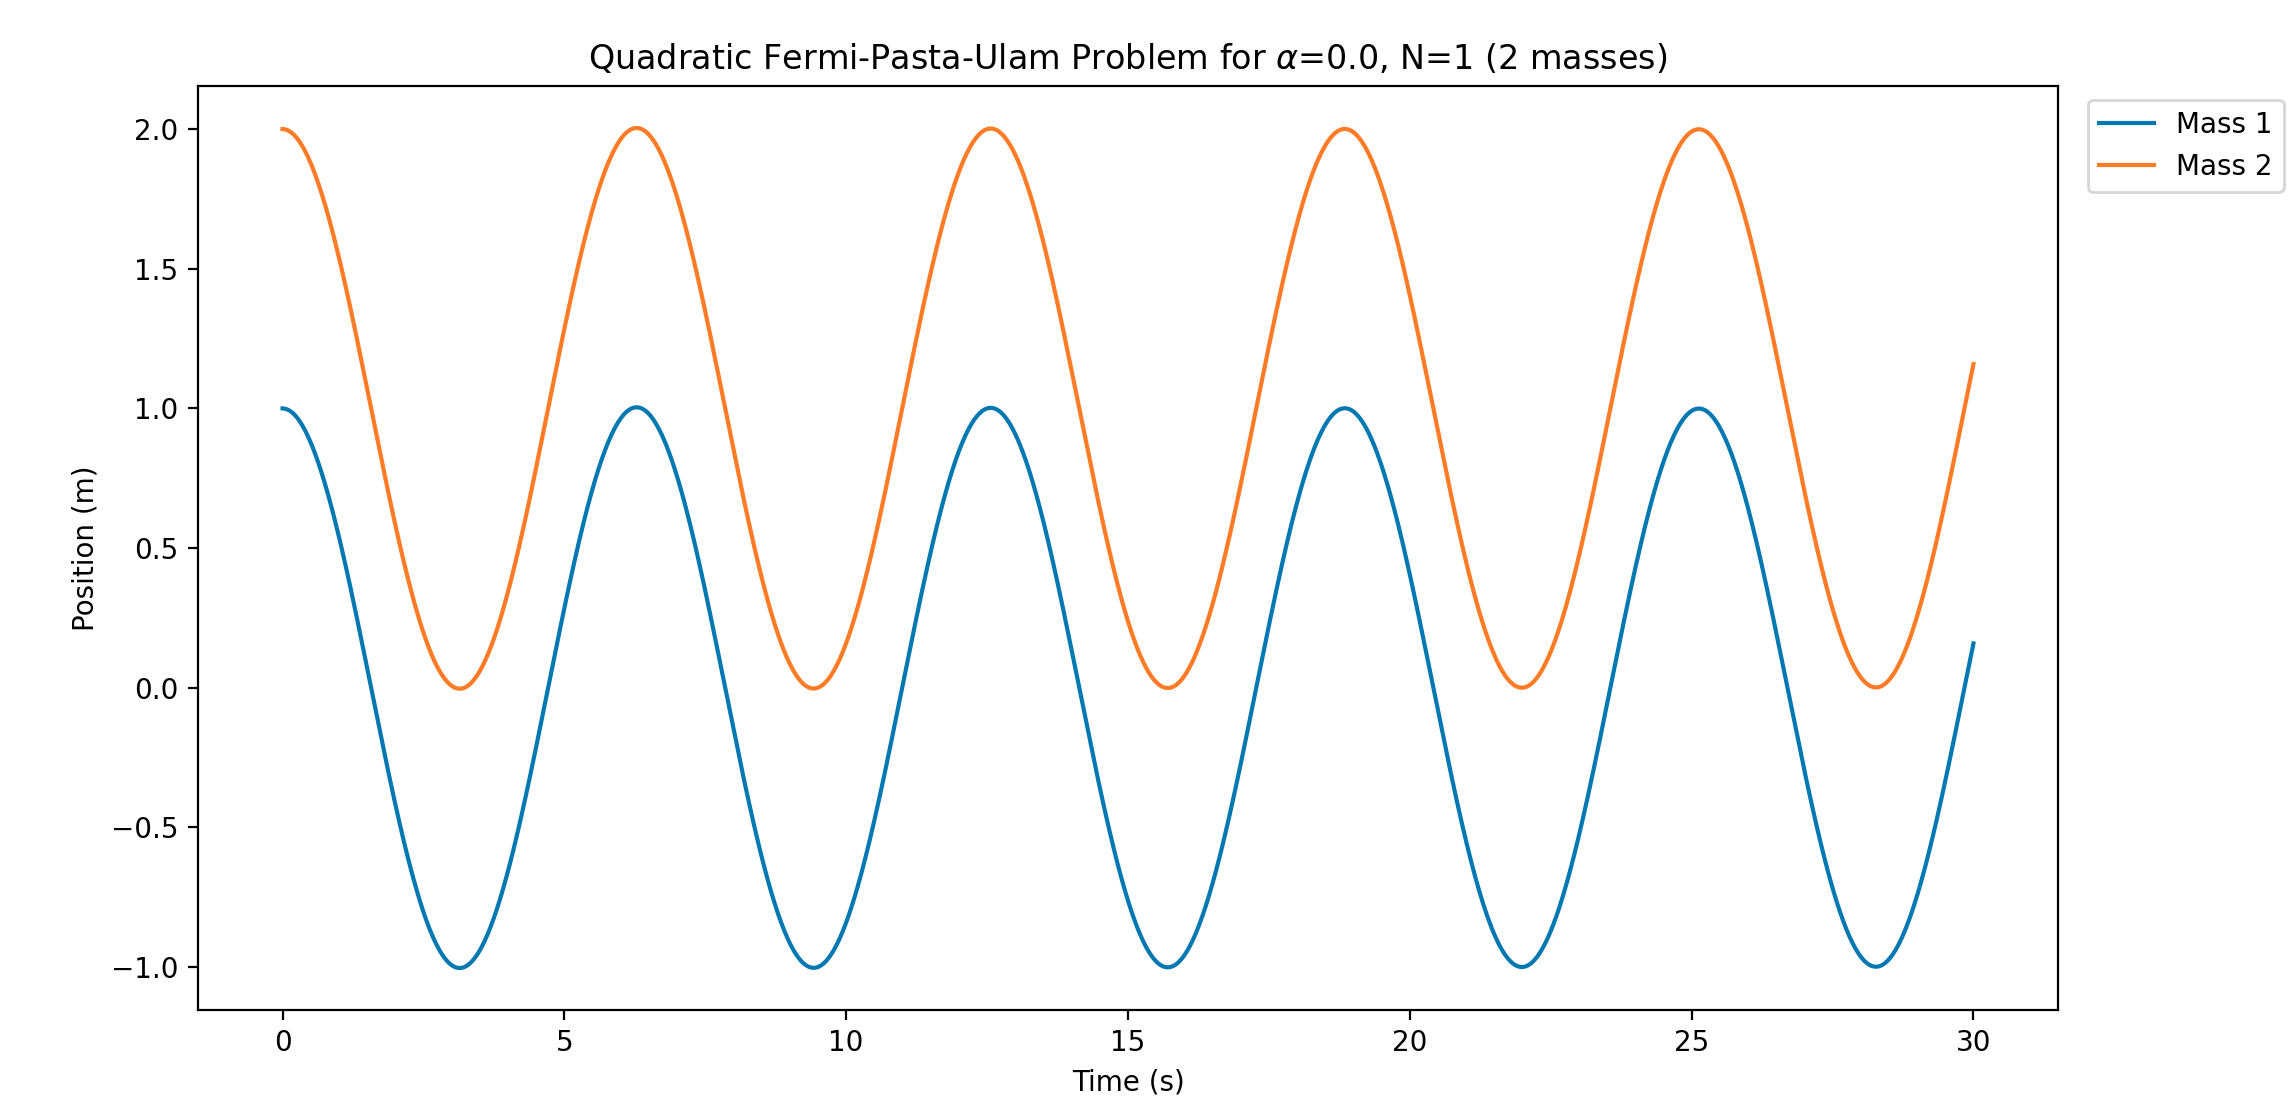
\includegraphics[scale=.33]{2mass.png}\\ 
    (Fig. 1)\\ 
    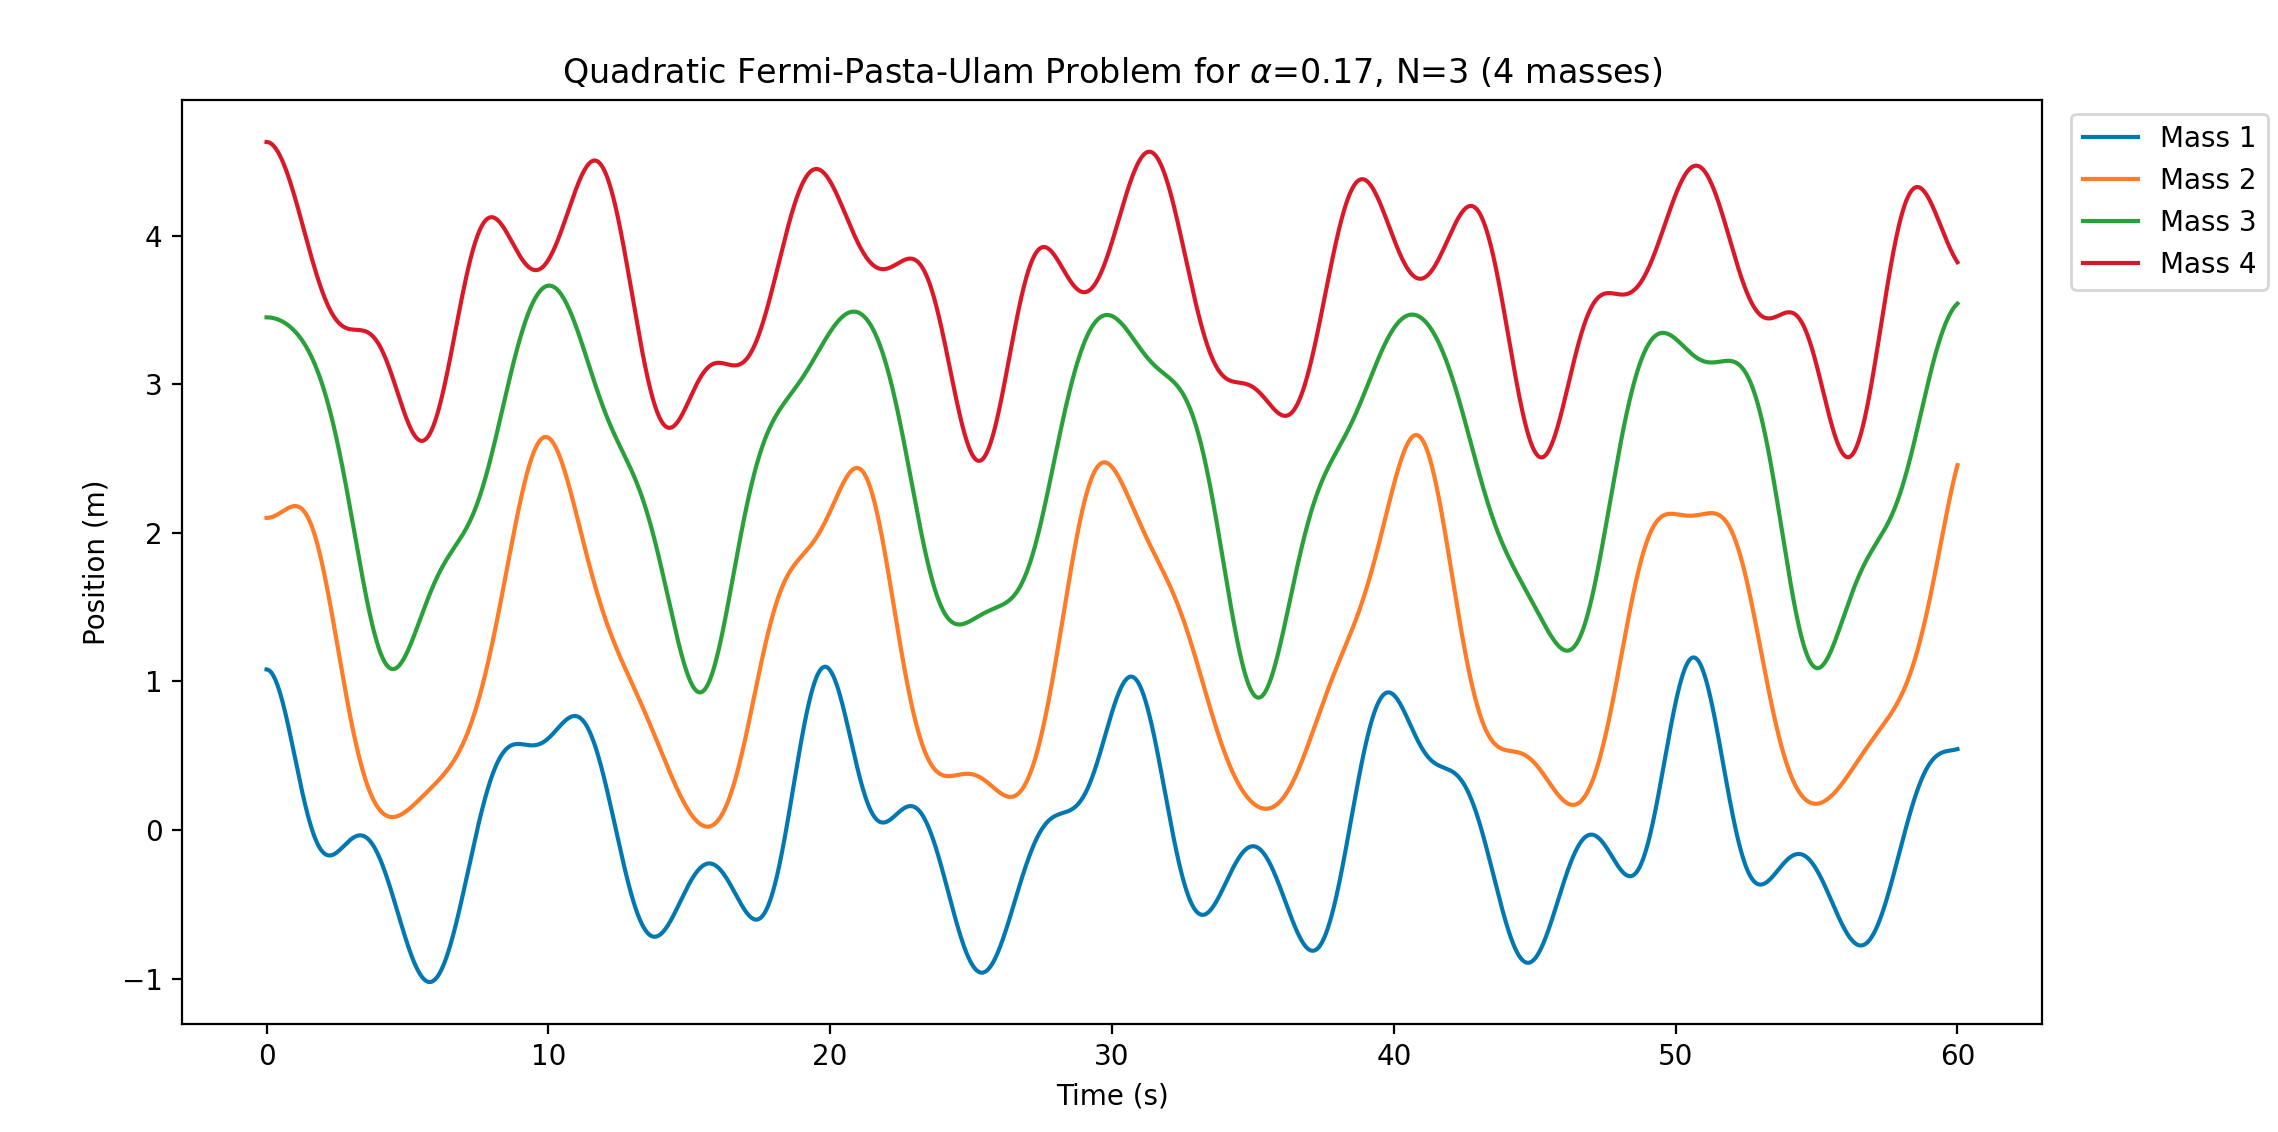
\includegraphics[scale=.33]{4mass.png}\\ 
    (Fig. 2)\\ 
    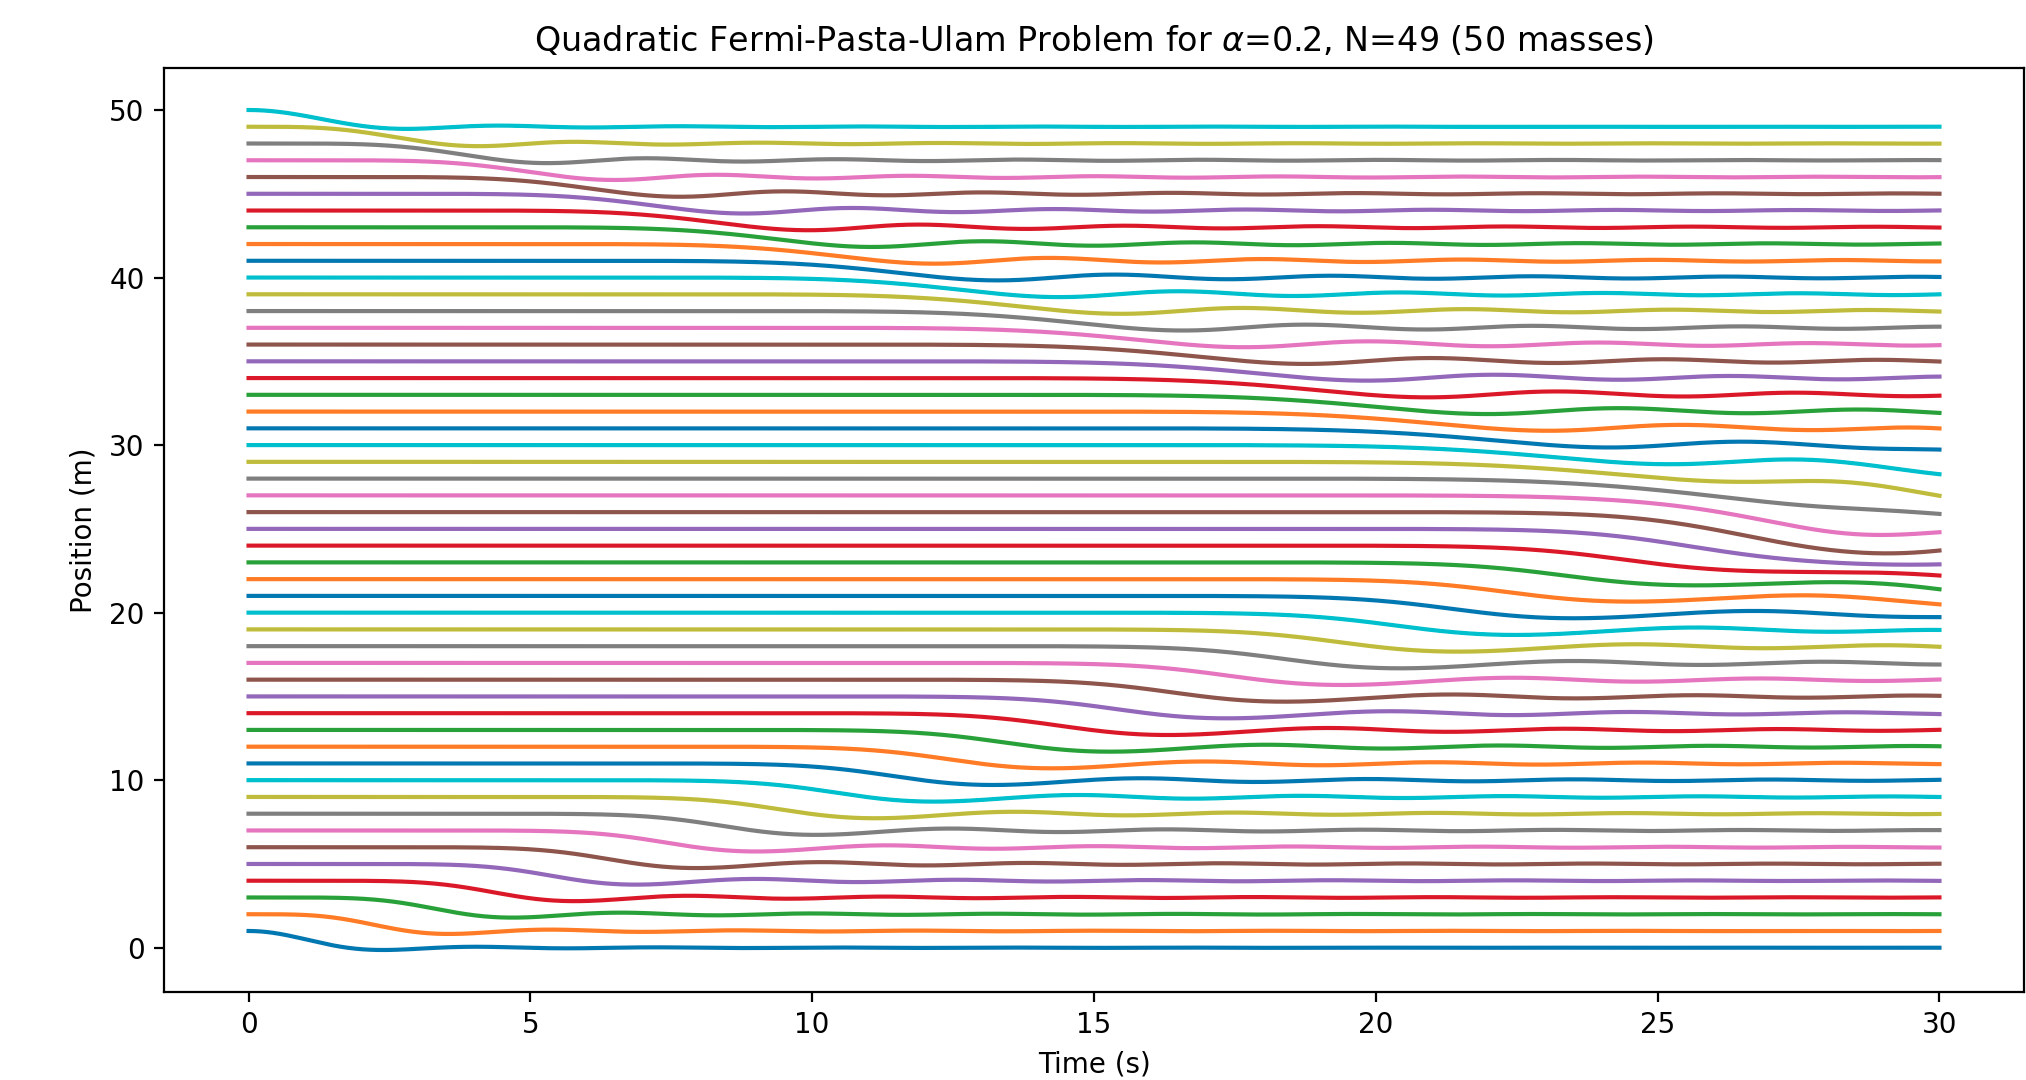
\includegraphics[scale=.33]{50mass.png}\\ 
    (Fig. 3)\\ 
    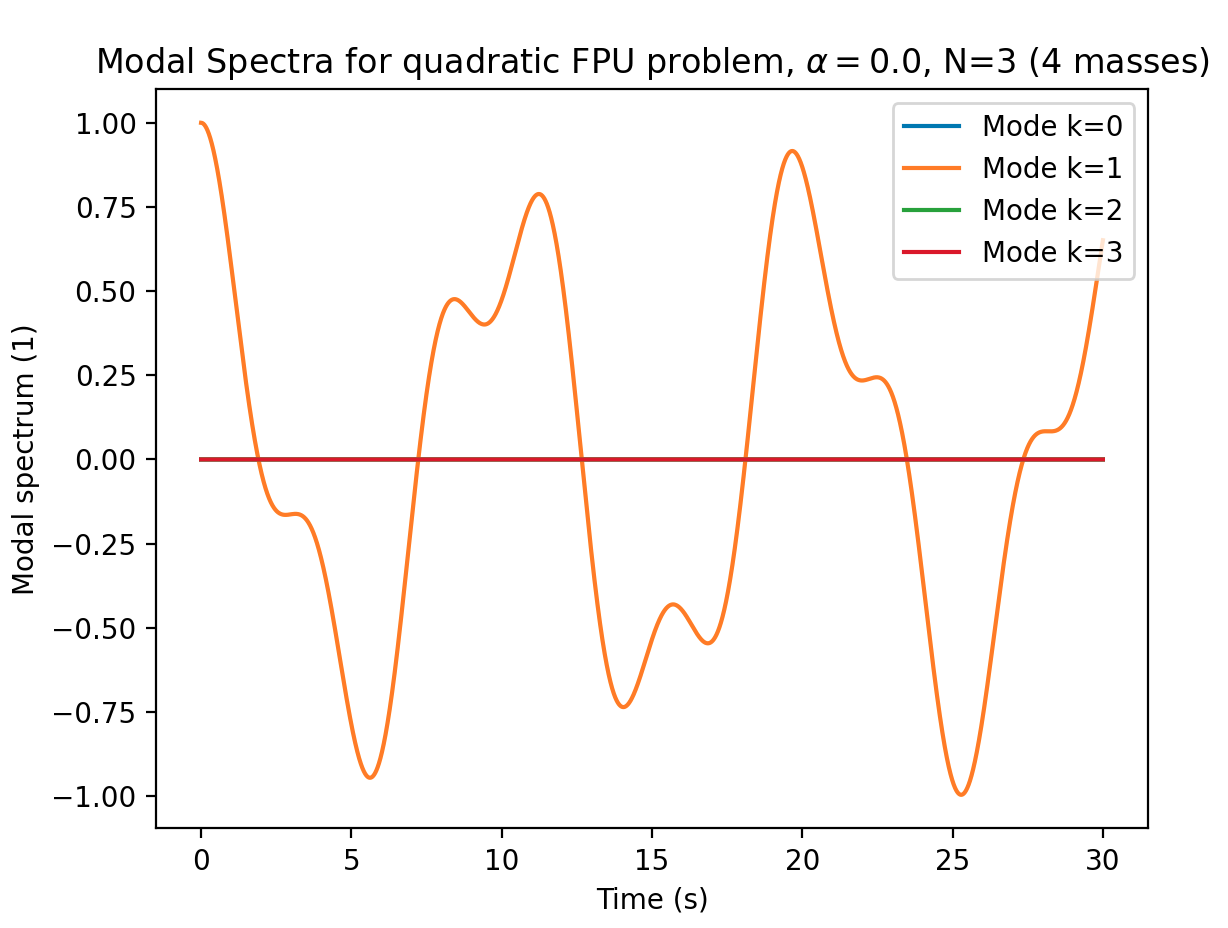
\includegraphics[scale=.5]{modea0k1.png}\\ 
    (Fig. 4)\\ 
    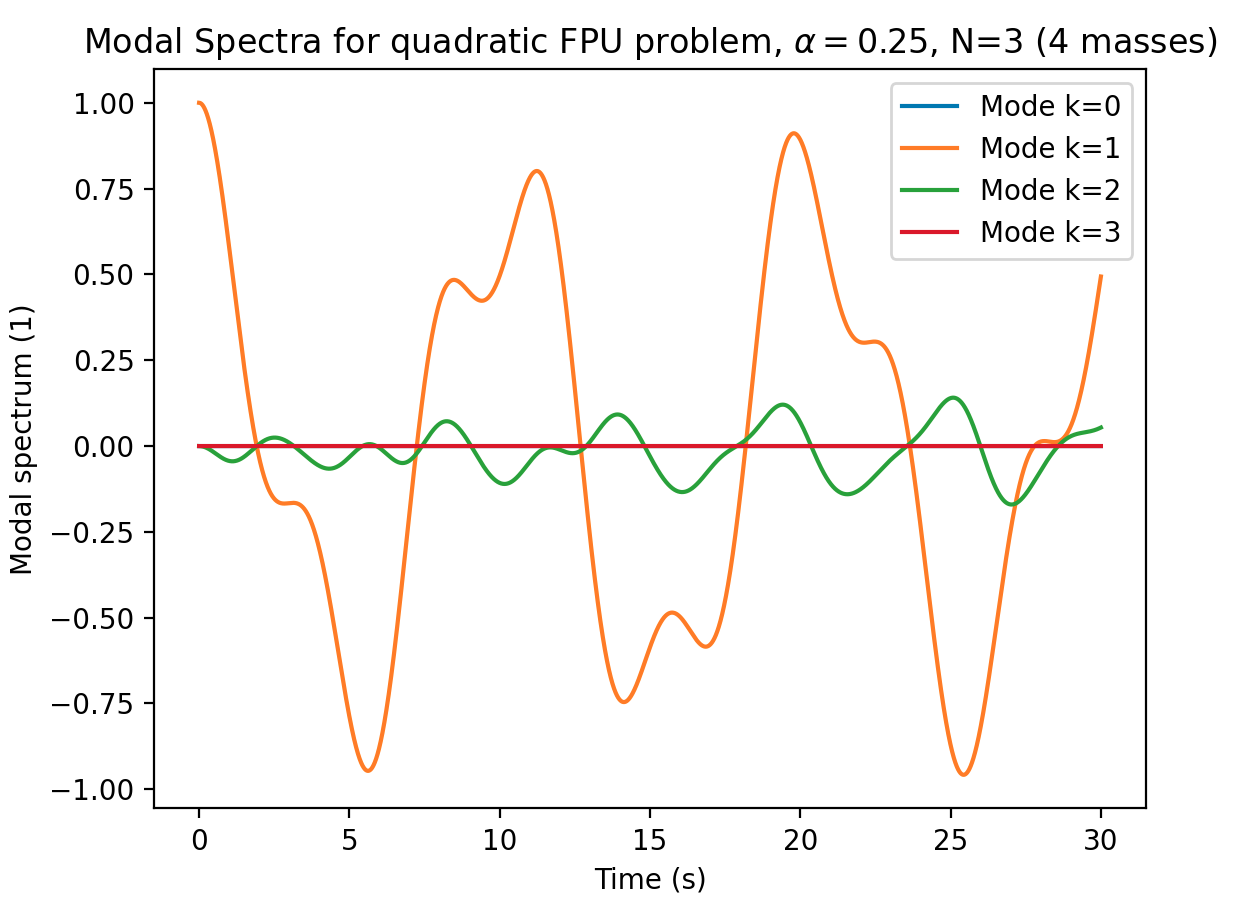
\includegraphics[scale=.5]{modea25k1.png}\\ 
    (Fig. 5)\\ 
    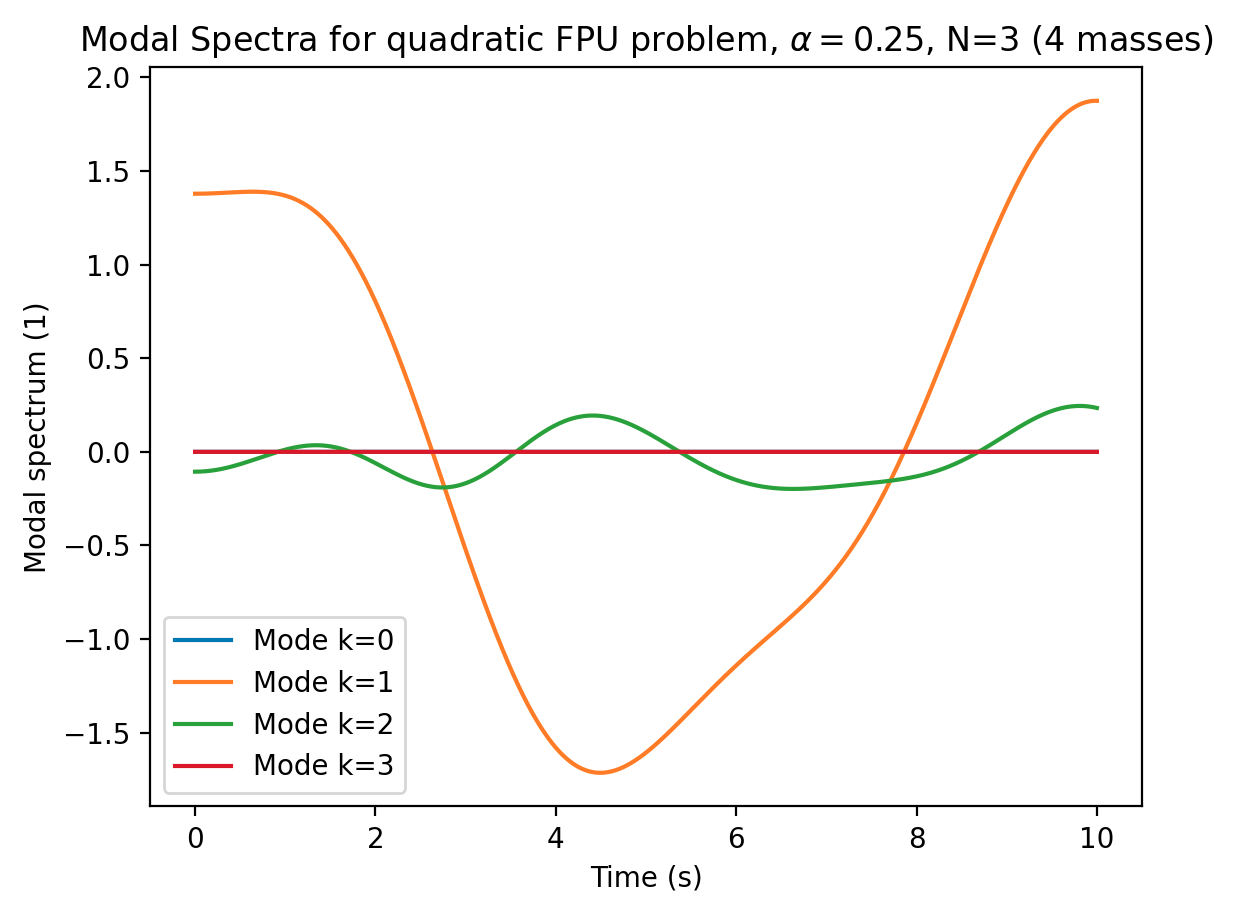
\includegraphics[scale=.5]{modea25arb.png}\\ 
    (Fig. 6)\\ 
    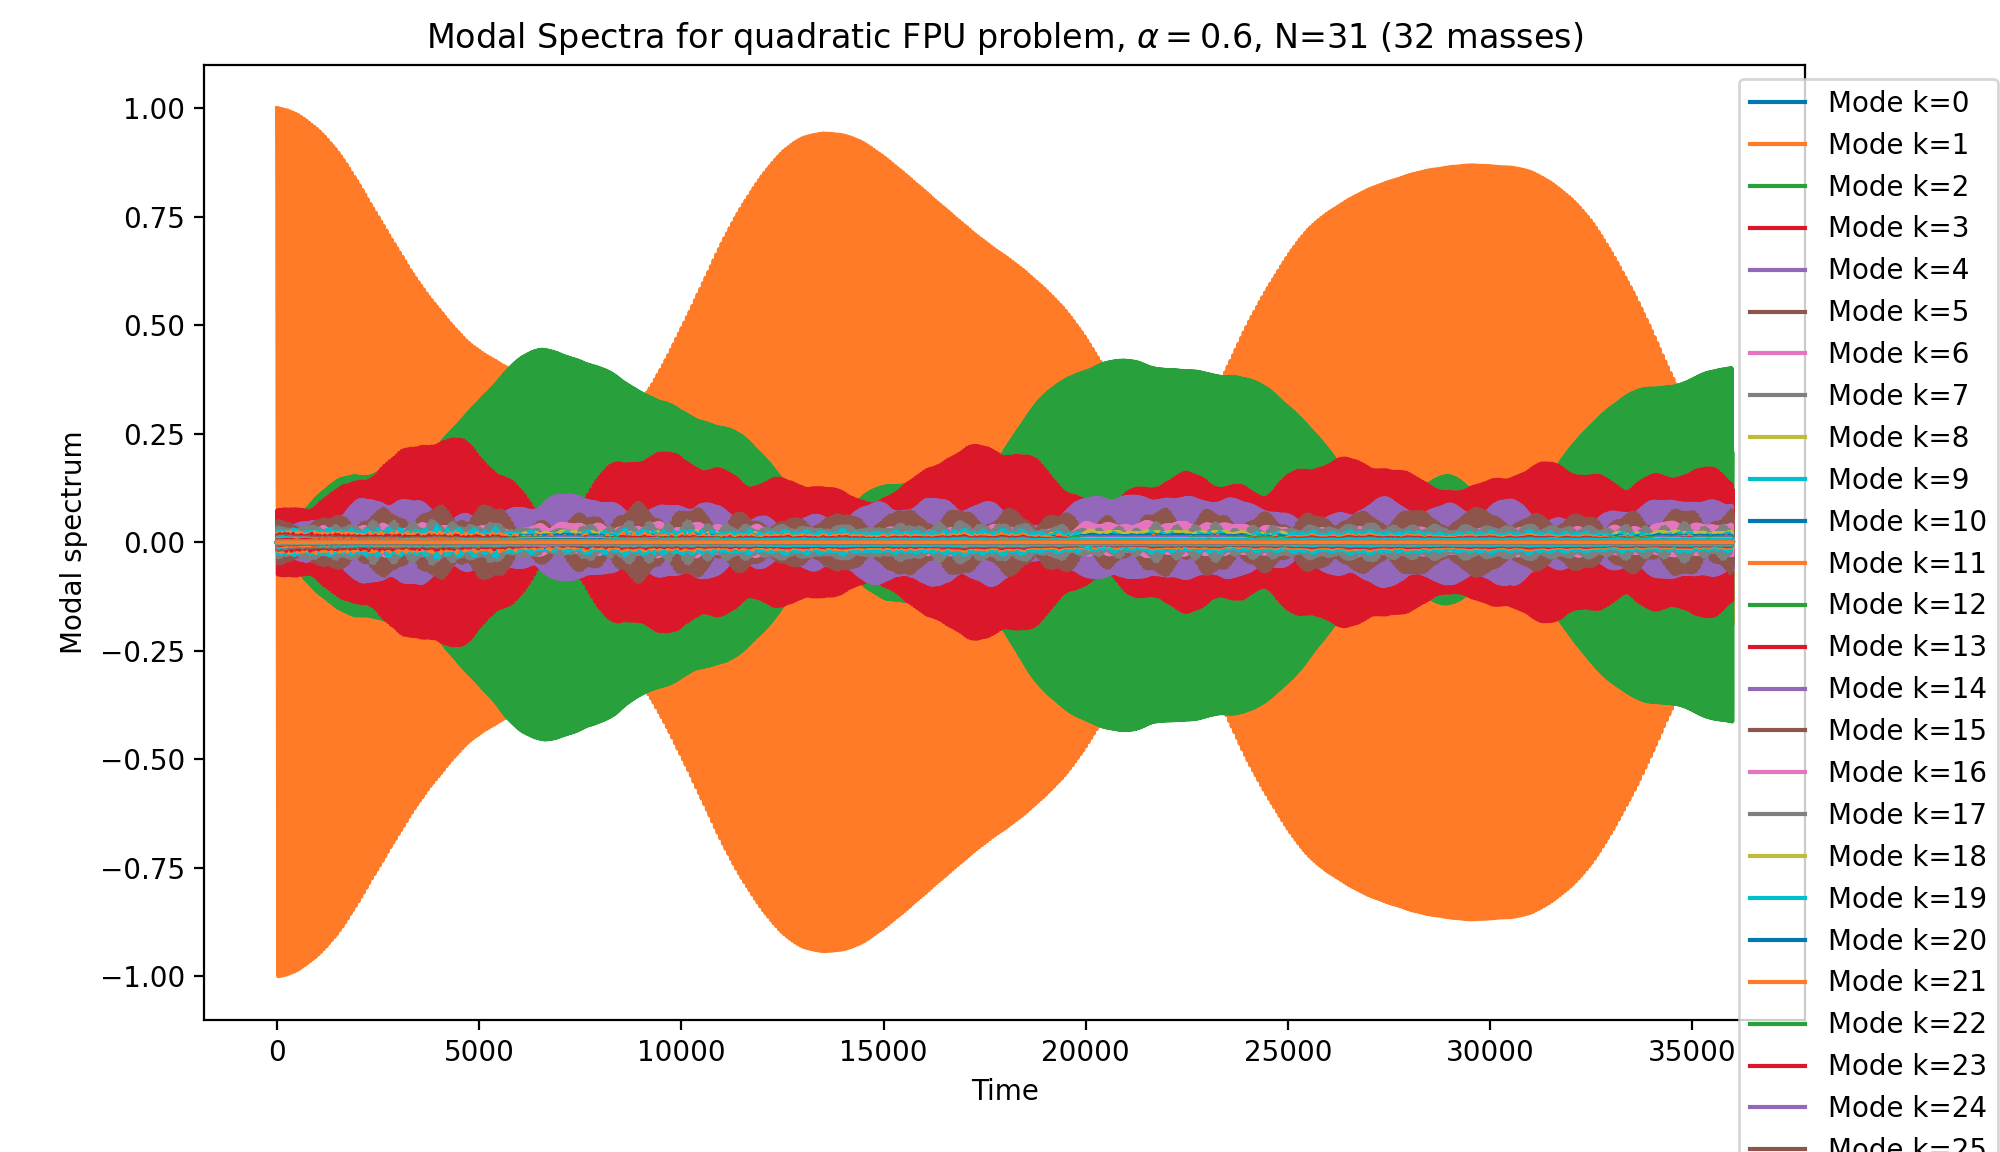
\includegraphics[scale=.36]{modea6k1.png}\\ 
    (Fig. 7)
    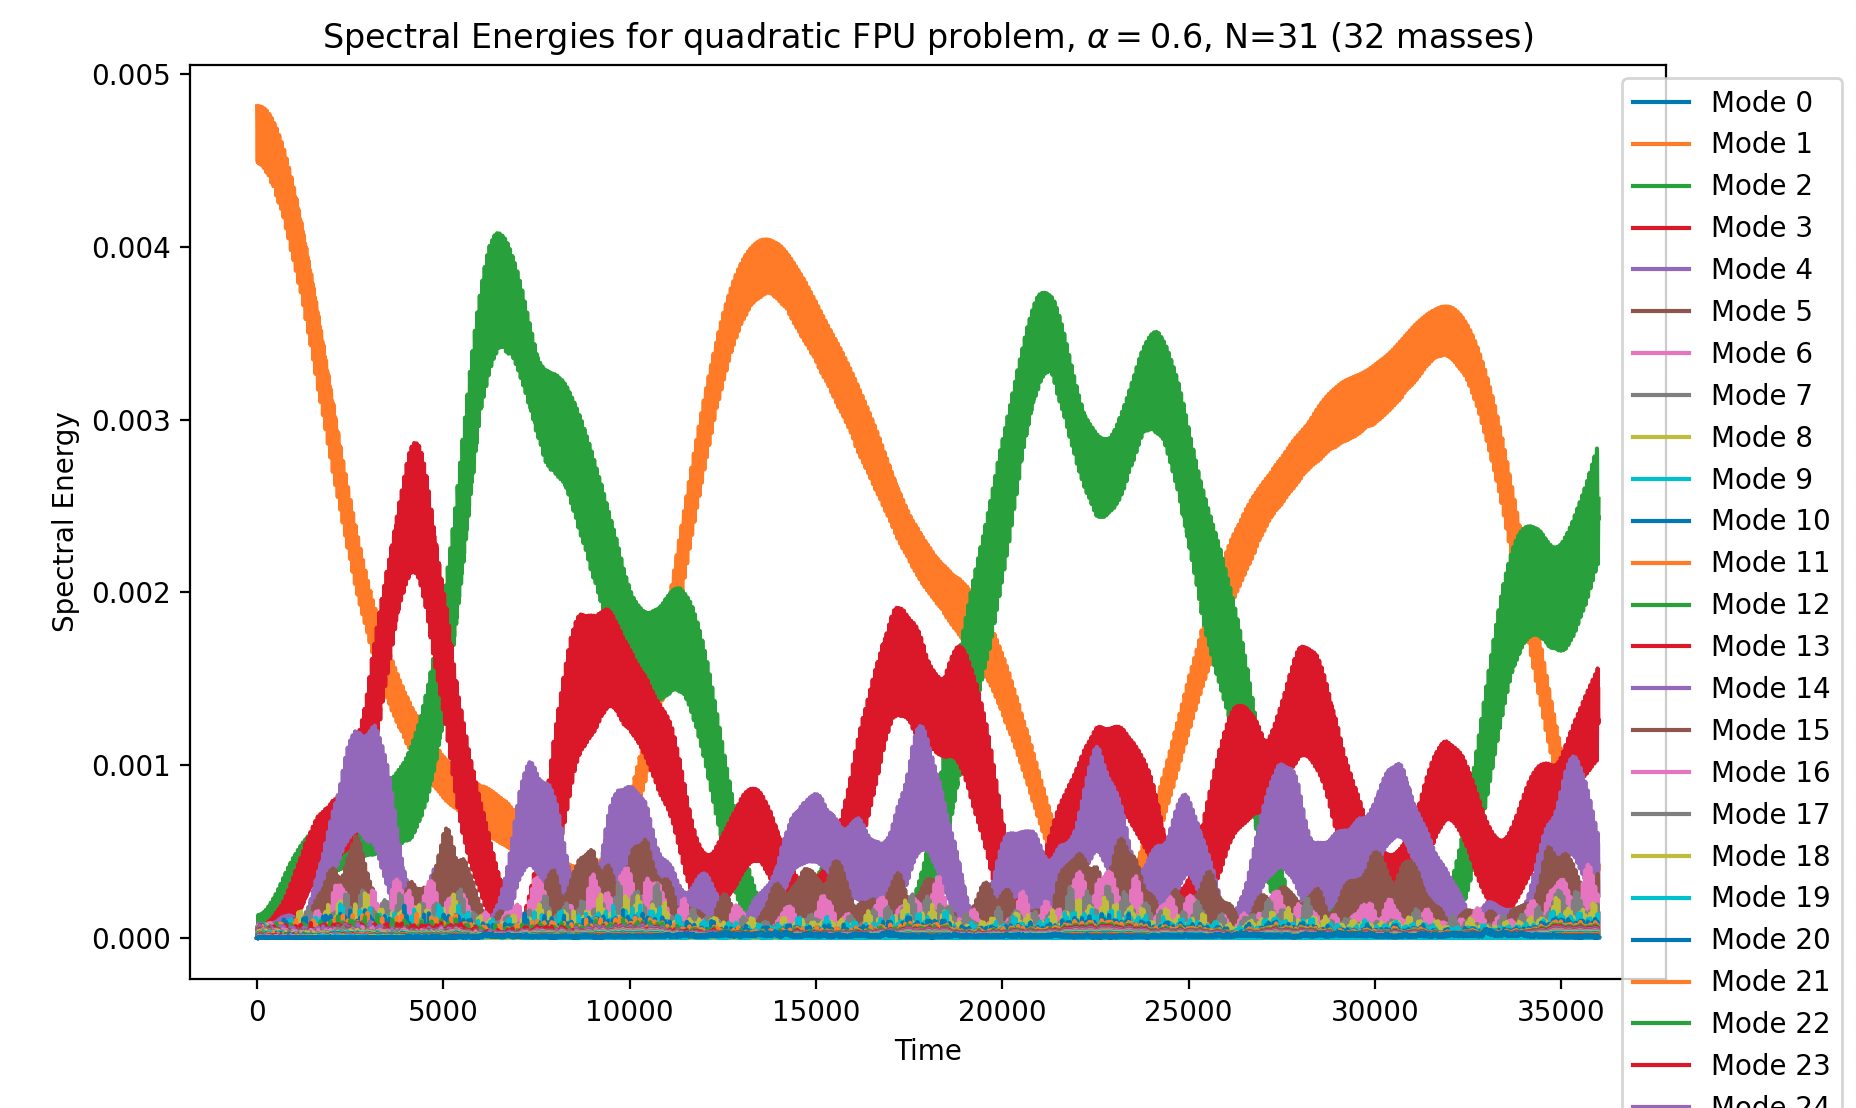
\includegraphics[scale=.36]{modeE.png}\\ 
    (Fig. 8)\\
    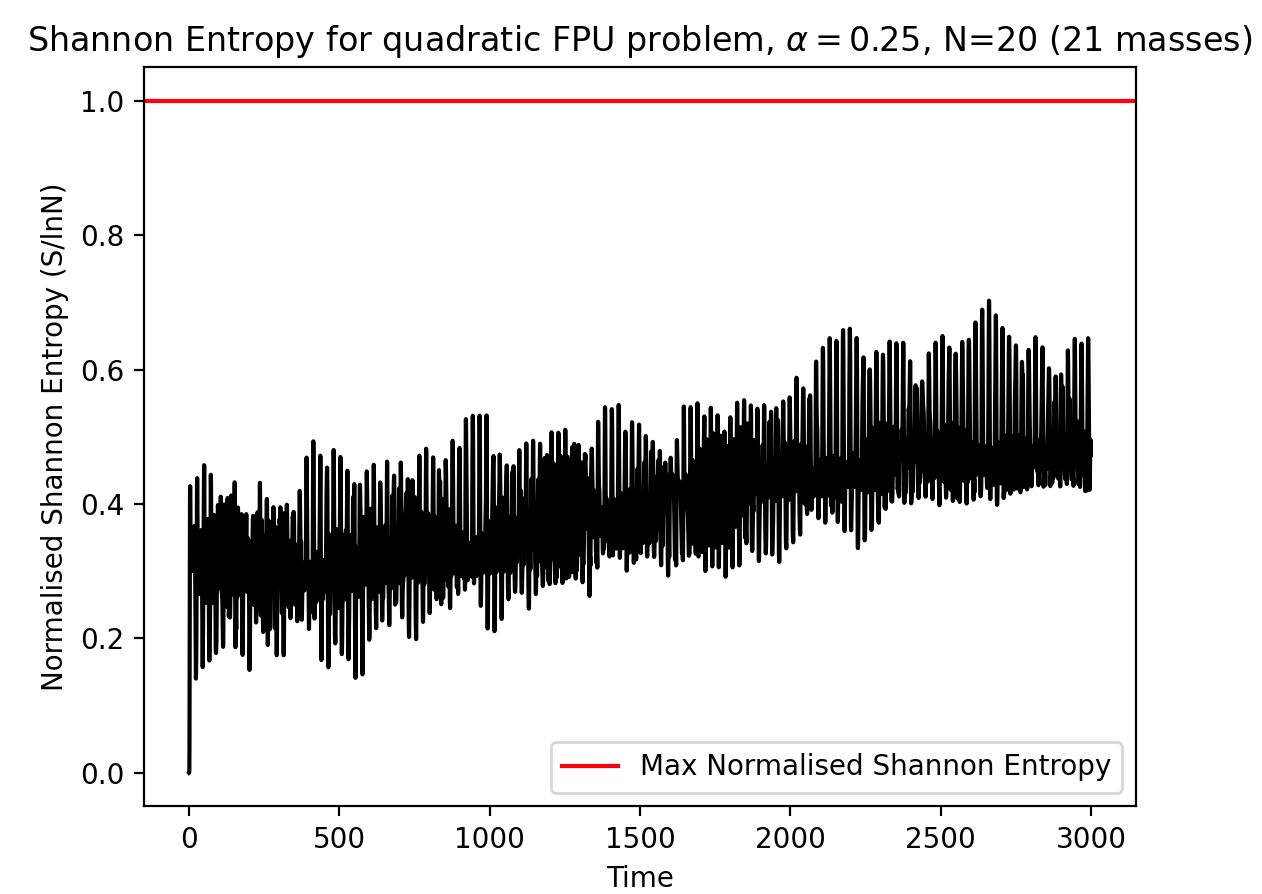
\includegraphics[scale=.6]{SEN20t3000.png}\\ 
    (Fig. 9)\\
    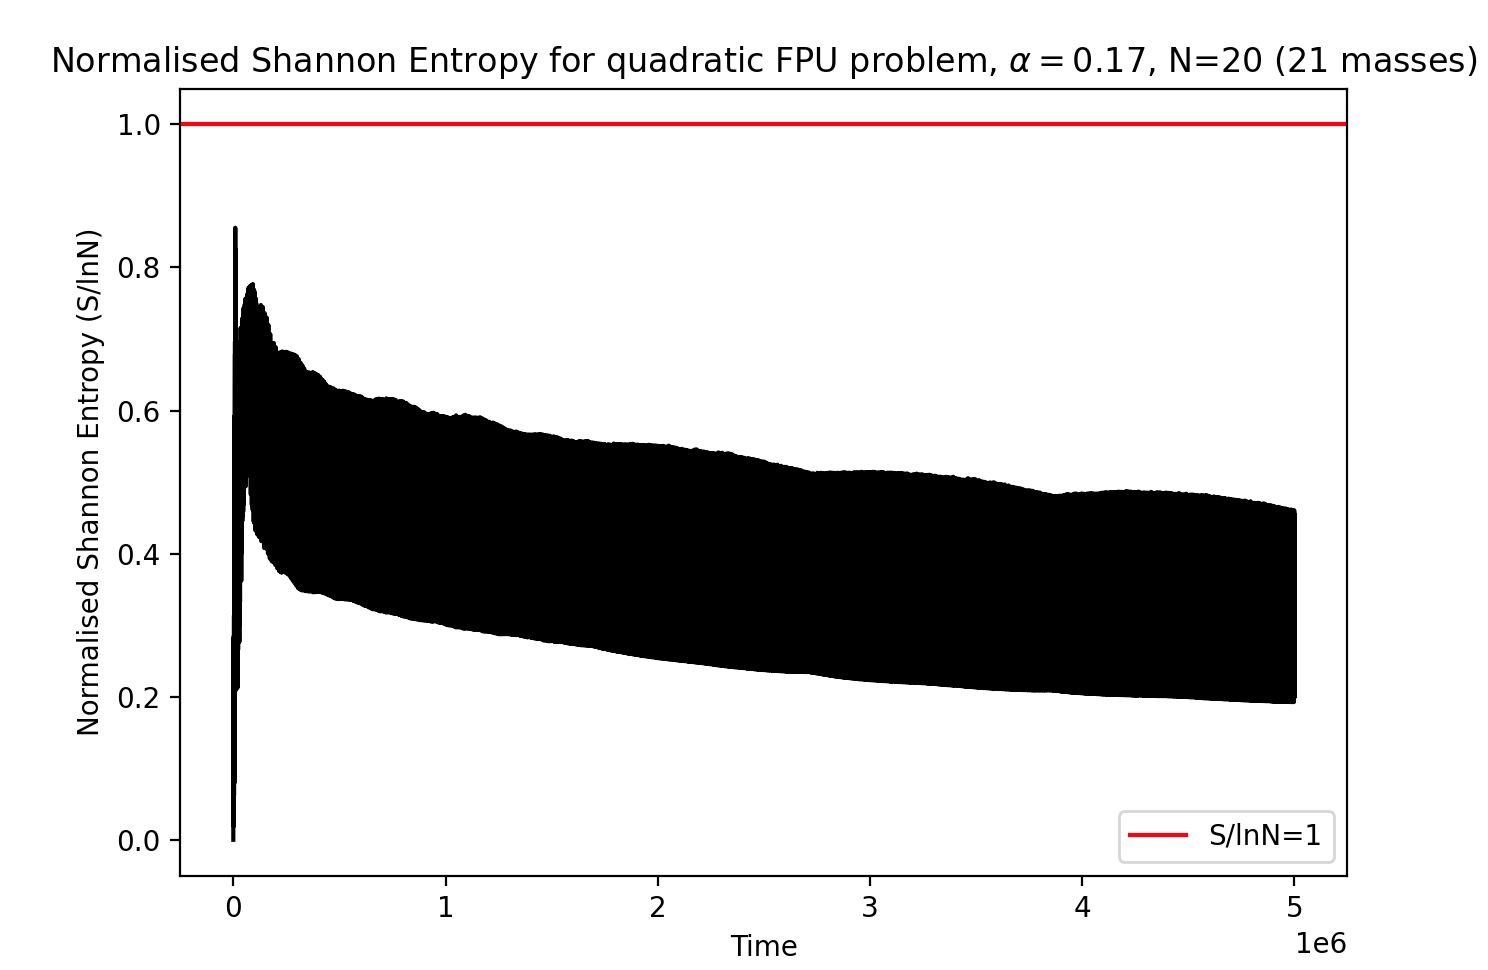
\includegraphics[scale=.5]{SEN20LT.png}\\ 
    (Fig. 10)\\
    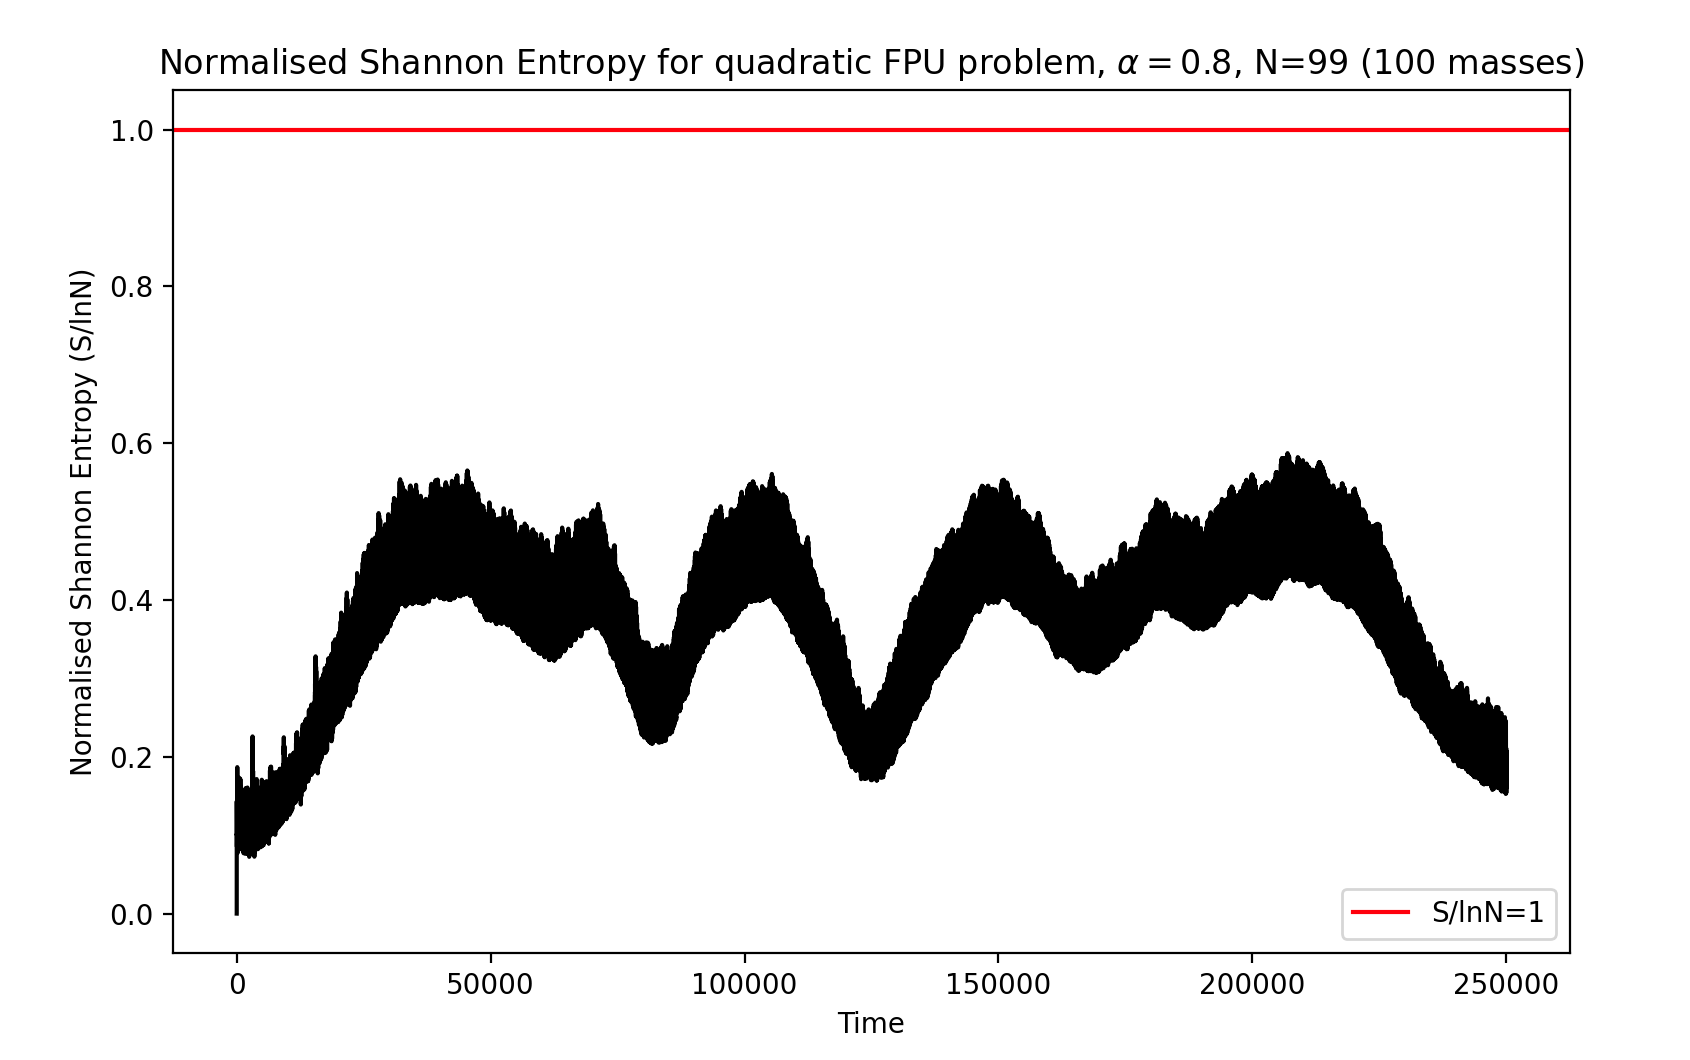
\includegraphics[scale=.45]{SEN100.png}\\ 
    (Fig. 11)\\ 
    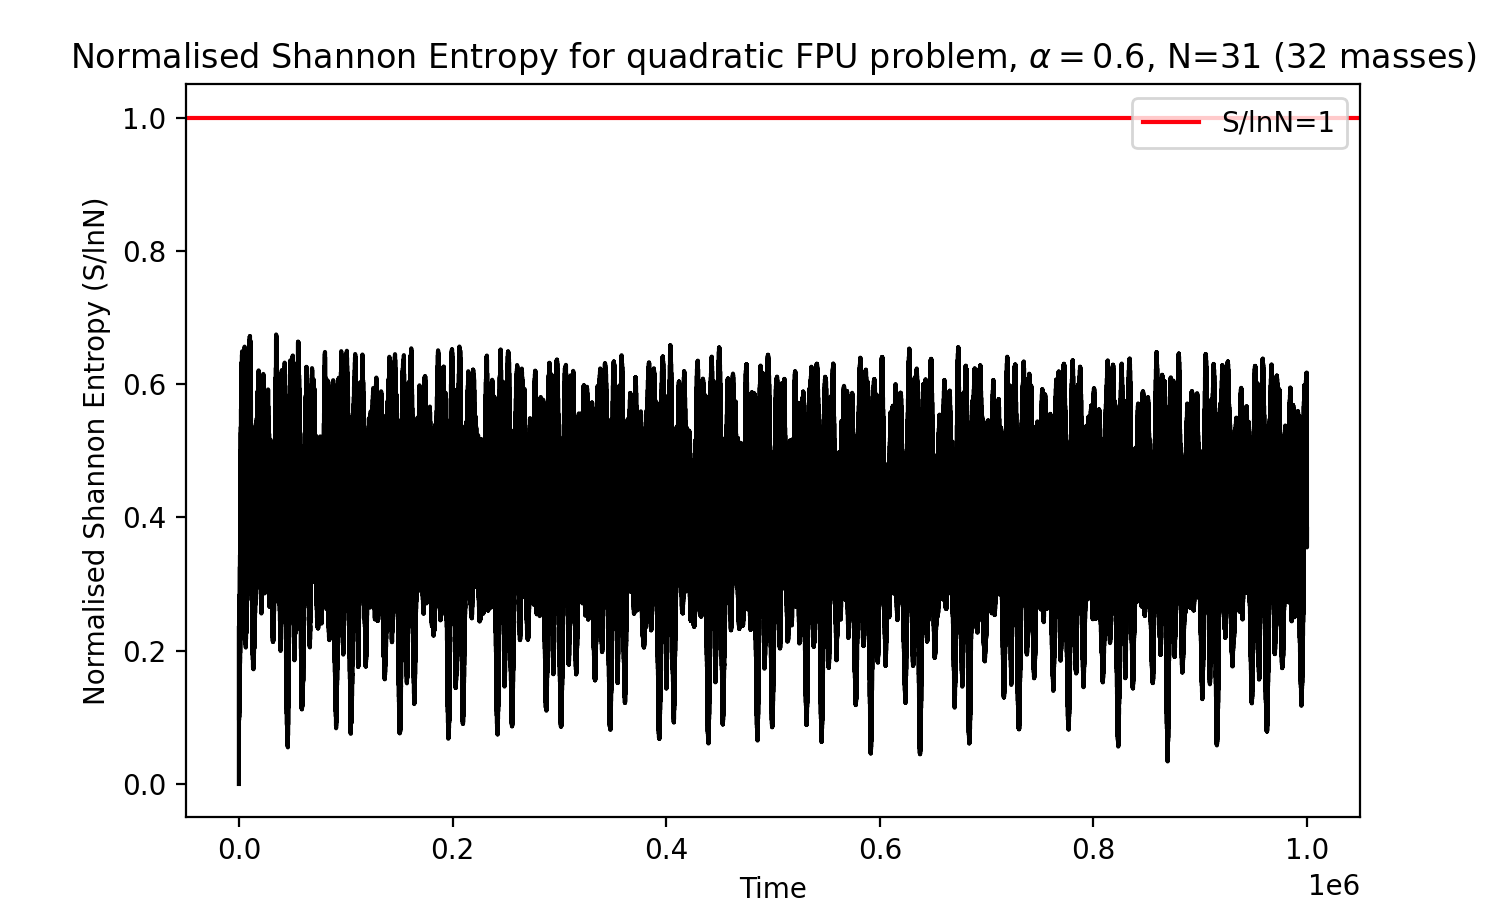
\includegraphics[scale=.5]{SEN32.png}\\ 
    (Fig. 12)
\end{center} 
\end{document}
